\documentclass{beamer} 
\usetheme{sts}
\usepackage{hyperref}
\pgfdeclareimage[height=1.2cm]{STS-logo}{STS-logo}
\logo{\pgfuseimage{STS-logo}}



\providecommand{\cpp}{C\kern-0.05em\texttt{+\kern-0.03em+} }
\providecommand{\Cpp}{\cpp}

%\usepackage{pdfpages}
\usepackage[utf8]{inputenc}
\usepackage[T1]{fontenc}
\usepackage{lmodern}
\usepackage{import}
\graphicspath{{../pics}}
%\usepackage{pgf}
%\usepackage{ctable}

\usepackage{listings}%[2000/08/23]
\usepackage{lstlangampl} % syntax file, I added some more keywords like 'display'

%\usepackage{graphicx}
%\usepackage{multicol}

%\usepackage{tikz}

\lstnewenvironment{cplus}
    {\lstset{language=c++,basicstyle=\scriptsize,frame=}}
    {}


\lstnewenvironment{cplus3}
    {\lstset{language=c++,basicstyle=\scriptsize,frame=}}
    {}


\lstnewenvironment{java}
    {\lstset{language=java,basicstyle=\scriptsize,frame=}}
    {}

\lstnewenvironment{java2}
    {\lstset{language=java,basicstyle=\scriptsize}}
    {}

\lstdefinelanguage{Haskell-custom}
{%columns=flexible,
escapeinside={--@}{@--},breaklines=true,breakatwhitespace=true%
language=Haskell,basicstyle=\color{lightblue}\ttfamily,keywordstyle=\ttfamily,%
morekeywords={class,instance,type,newtype,data,where,deriving,import},%
lineskip=-.1\baselineskip,morekeywords={concept,requires,concept_map}}

\lstnewenvironment{hask}[1][\small]{\lstset{language=Haskell-custom,%
    style=numbers,basicstyle=\color{lightblue}#1\ttfamily,keywordstyle=#1\ttfamily,%
    style=bold-keywords,style=frametb}}{}

\providecommand{\haskellinl}[2][\normalsize]{{\lstinline[language=Haskell-custom,%
basicstyle=\color{lightblue}#1\ttfamily,keywordstyle=#1\ttfamily]@#2@}}%

\providecommand{\haskinl}[2][\normalsize]{{\lstinline[language=Haskell-custom,%
basicstyle=\color{lightblue}#1\ttfamily,mathescape=true,keywordstyle=#1\ttfamily]@#2@}}%

\lstdefinestyle{markers}{rangeprefix=\{-\:\ ,%
includerangemarker=false,%
rangesuffix=\ \:-\}}%

\providecommand{\haskellinput}[3][\small]{{\lstinputlisting[language=Haskell-custom,basicstyle=\color{lightblue}#1\ttfamily,keywordstyle=#1\ttfamily,%
style=bold-keywords,style=numbers,style=frametb,style=markers,firstnumber=1,linerange={#3}]{#2}}}

\providecommand{\haskellinputnonumber}[3][\small]{{\lstinputlisting[language=Haskell-custom,basicstyle=\color{lightblue}#1\ttfamily,keywordstyle=#1\ttfamily,%
style=bold-keywords,style=frametb,xleftmargin=8pt,xrightmargin=8pt,style=markers,firstnumber=1,linerange={#3}]{#2}}}



\title[Automated Unit Test Generation]{Automated generation of Unit Tests from UML Activitys using the AMPL interface for Constraint Solvers } 
\subtitle[Short Subtitle]{Long Subtitle} 
\author[F. Kurth]{Felix Kurth} 
\day=13
\month=8
\year=2013
\date[\today]{\today} 

\AtBeginSection[] % Do nothing for \section*
{
\begin{frame} 
\frametitle{Outline} \tableofcontents[currentsection]
\end{frame}
}

\begin{document}

%\begin{frame}
%\titlepage
%\end{frame}
%
%\begin{frame}
%\frametitle{Outline} 
%\tableofcontents  
%\end{frame}
%
%
%\section{Motivation}
%
%\lecture{Airbus Specific Content}{airbus}
%\subsection{Model Based Engineering at Airbus}
%\begin{frame}
%\frametitle{Generating C-Component Code and Unit test Code from the same Model}
%%\def\svgwidth{300pt} \import{../pics/}{Activity2Code+Testsfaster.pdf_tex}
%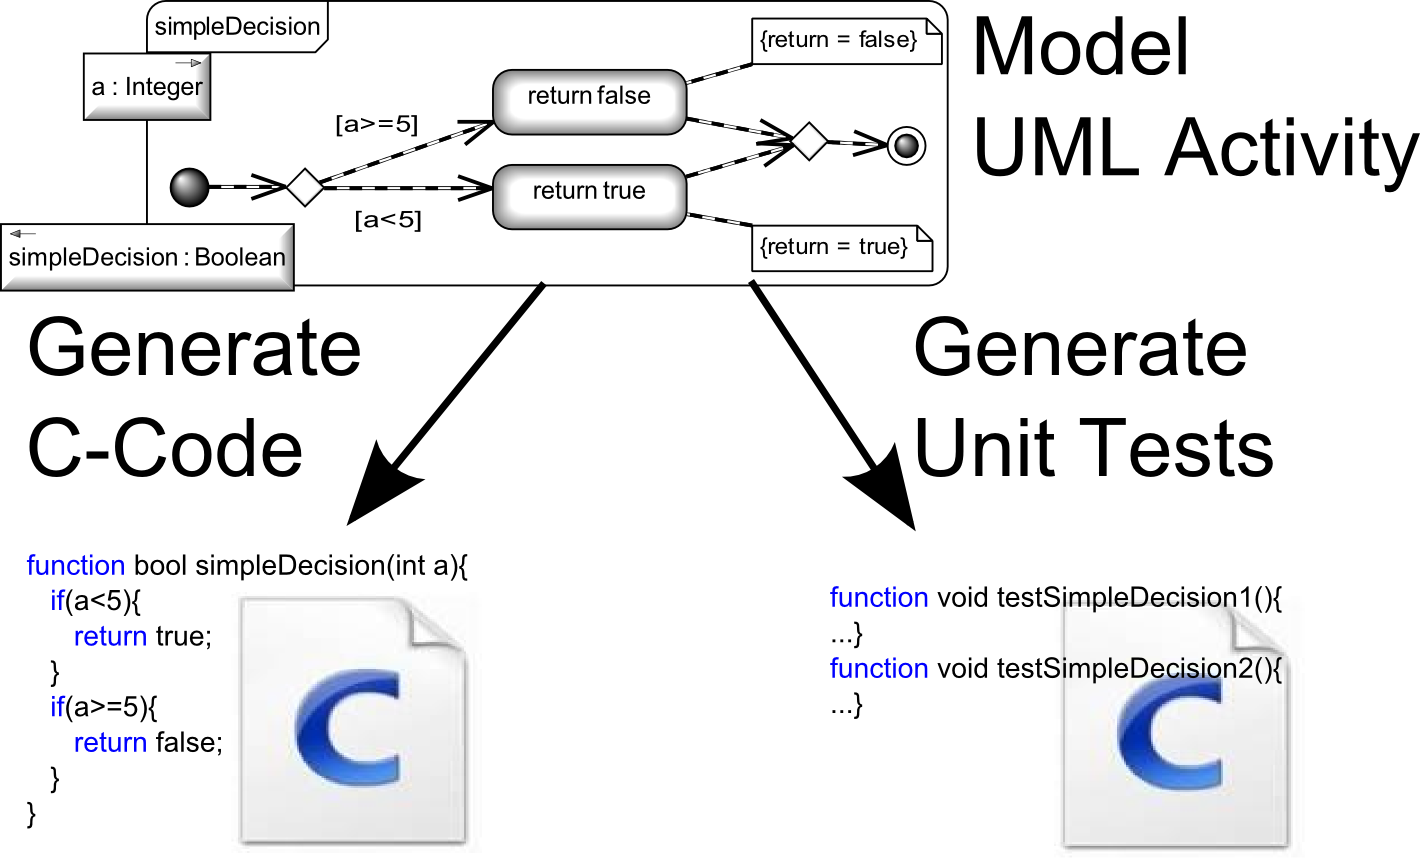
\includegraphics{../pics/Activity2Code+Tests.png}
%%\import{{Activity2Code+Tests.pdf_tex}}
%\end{frame}
%
%\begin{frame}
%\frametitle{Independence of Implementation- and Test-model} 
%\begin{itemize} 
%\item Artisan Automated Code Synthesis generates C Implementation from UML Activities
%\item C Unit tests shall be generated from the same Model
%\item Use OCL to specify LocalPostConditions and Guard conditions used for Test Generation
%\item The structure of the Control Flow Graph is shared between Implementation and Testmodel
%\end{itemize}
%\end{frame} 
%
%\begin{frame}
%%stupid Logo frame
%here you could see some logos of Artisan Airbus and a screen-shot
%\end{frame}
%
%
%\lecture{Introduction}{intro}
%\subsection{Developing Tool generating Unit Tests from UML Activities}
%\begin{frame}
%\frametitle{Overall Goals of this Thesis}
%\begin{itemize}
%\item Develop a demonstration tool producing test stimuli from UML Activities %could be problem
%\item Integrate with existing test generating plug-in for Eclipse
%\item Focus on C-Component Architecture
%\item Use AMPL interface for constraint solvers
%\item provide extensible architecture
%\item use Eclipse Modeling Framework (EMF) standard technology
%\end{itemize}
%\end{frame}
%
%\begin{frame}
%\frametitle{The Overall Work Flow of Generating Unit Tests from a Model}
%\begin{block}{Normalisation}
%Resolve ambiguities in UML representation and semantic
%Making implicit assumptions explicit
%\end{block}
%\begin{block}{AMPL Modeling}
%Convert model into a form that is understood by constraint solvers
%\end{block}
%\begin{block}{Abstract Testcase Generation}
%Produce an effective suite of relevant test cases
%\end{block}
%\begin{block}{Producing Concrete Unit Tests}
%Find boundary values
%Output Unit Tests
%\end{block}
%\end{frame}
%
%\subsection{Introductory Example}
%\begin{frame}[fragile]
%\frametitle{Introductory Example}
%\begin{columns}
% \column{.45\textwidth} \ 
%	\begin{block}{Specifying a Path} 
%	\def\svgwidth{\textwidth}
%	\scriptsize
%	\import{../pics/}{SomeActivityDiagramsSimpleDecision.pdf_tex}
%%\includegraphics[scale=\textwidth]{../pics/SomeActivitySimple}
%	\end{block} 
%\column{.5\textwidth} \ 
%	\begin{block}{AMPL} 
%		\begin{lstlisting}[basicstyle=\ttfamily\scriptsize,language=ampl]
%param l; #Pathlength
%set t default {}; #True
%set f default {}; #False
%set d2f default {}; #d2false
%set d2t default {}; #d2true
%
%# Variables can be Properties, 
%# Parameters, Local Variables uvm.
%var a{0..l} : integer; 
%var r{0..l} in {0,1}; #Boolean
%
%# Constraints
%s.t. t_post1{i in t}: r[i]=1;
%s.t. t_post2{i in t}: a[i]=a[i-1];
%s.t. f_post1{i in f}: r[i]=0;
%s.t. f_post2{i in f}: a[i]=a[i-1];
%s.t. f_guard{i in d2f}: a[i]<=5;
%s.t. t_guard{i in d2t}: a[i]>=6;
%\end{lstlisting}
%	\end{block} 
%\end{columns}
%\end{frame}
%
%\begin{frame}[fragile]
%\frametitle{Introductory Example}
%	\begin{block}{Specify Path} 
%		\begin{lstlisting}[basicstyle=\ttfamily\scriptsize,language=ampl]
%param l:= 1; # Path contains one Action
%set d2f:= 0; # d2false Guard
%set f:= 1; # False Action
%		\end{lstlisting}
%	\end{block} 
%	\begin{block}{Result} 
%		\begin{lstlisting}
%LP_SOLVE 4.0.1.0: optimal, objective 0
%0 simplex iterations
%:   a  return    :=
%0   -5    0
%1   -5    0
%;
%		\end{lstlisting}
%	\end{block}
%\end{frame}
%
%
%%\begin{frame}
%%\frametitle{The Overall Work flow of Generating Unit test from a Model}
%%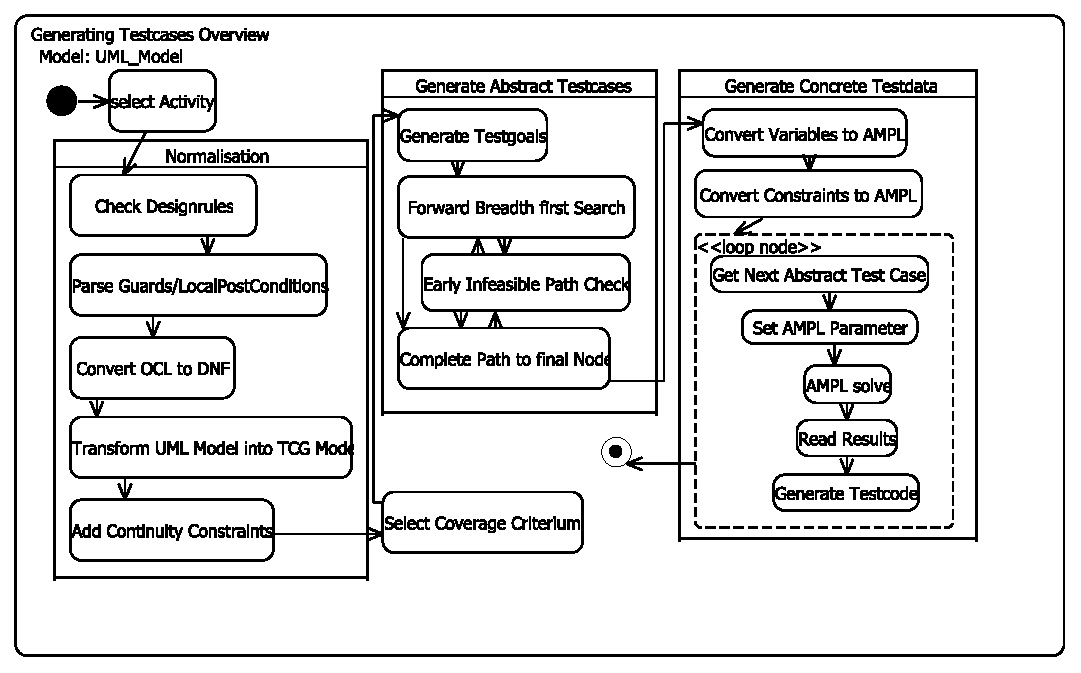
\includegraphics[scale=0.6]{../pics/Workflow.pdf} 
%%\end{frame}
%
%%\subsection{Goals of the Tool Development}
%%\subsubsection{Normalisation}
%%\begin{frame}
%%\frametitle{Why do we need Normalisation?}
%%\begin{itemize}
%%\item Filling in Semantic Variation Points	%Action is mapped to a C Codeblock, Semantic of Parameters
%%\item Removal of unnecessary details		%copy only referenced Variables, Remove Namespaces
%%\item Removing ambiguous Representations	%OwnedRule instead of LocalPostconditions
%%\item Making implicit assumptions explicit 	%else, Continuity Constraints, context Operation
%%\end{itemize}
%%\end{frame}
%%
%%\subsubsection{Coverage Criteria and Abstract Testcases}
%%\begin{frame}
%%\frametitle{Requirements for Abstract Testcase generation}
%%\begin{itemize}
%%\item Produces an effective suite of relevant test cases
%%\item Supports a variety of Coverage Criteria
%%\item Do not get stuck in loops or combinatorial explosion
%%\item eliminate infeasible paths as early as possible
%%\end{itemize}
%%\end{frame}
%%
%%\begin{frame}
%%\frametitle{Definition of Abstract Test Cases}
%%%an abstract testcase is one specific Path and potentially Additional constraints specifiying valueassignments of subexpressions.
%%\end{frame}
%%
%%\subsubsection{Constraint Solving for Specific Test Stimuli}
%%\begin{frame}
%%\frametitle{Wish List for Generating Specific Values}
%%\begin{itemize}
%%\item Support for a large subset of OCL specification
%%\begin{itemize}
%%\item Arithmetic constraints (linear and non-linear)
%%\item Set expressions and operations
%%\item Object type variables
%%\end{itemize}
%%\item Efficient algorithms for variety of constraint systems
%%\item Interchangeability of Constraint Solvers
%%\end{itemize}
%%\end{frame}
%
%
%\section{Generating Test Cases Step by Step}
%\subsection{Activity Test Case Graph}
%\begin{frame}
%\frametitle{Activity Test Case Graph}
%\begin{itemize}
%\item An Activity contains Nodes, Edges and Variables
%\item Nodes are supplied with multiple LocalPostconditions (OCL Expressions)
%\item An Edge has exactly one Guard Condition (OCL Expressions)
%\item Variables are referenced by OCL Expressions 
%\item Variables can be changeable (Local Variables, Properties) or fixed (Parameters, constant Properties)
%\item Variables can be Basic Variables (Integer, Boolean, Float) or Compound Variables (Collection, Object)
%\item \emph{Activity Test Case Graph} is a refinement of the more General \emph{Abstract Test Case Graph} Meta Model
%\end{itemize}
%\end{frame}
%
%\begin{frame}
%\frametitle{The Activity Test Case Graph Class Model}
%	\def\svgwidth{\textwidth}
%	\tiny
%	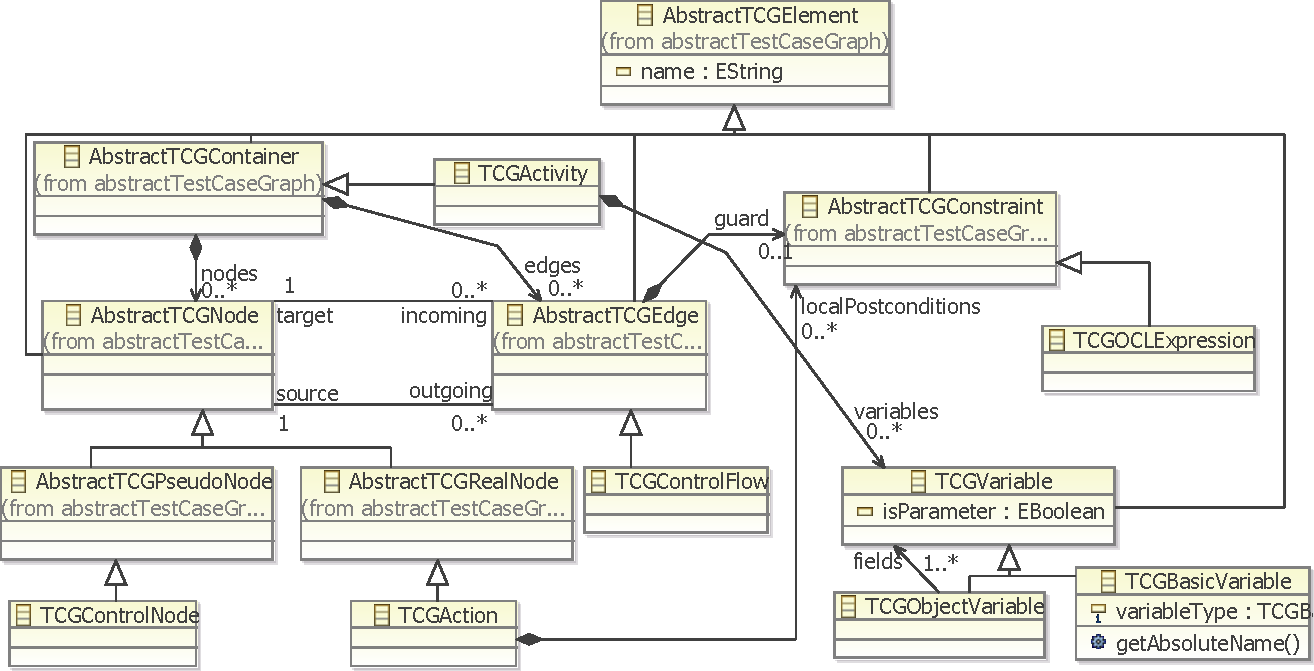
\includegraphics[width=\textwidth]{../pics/completeMetamodelforSlideshowN.pdf}
%\end{frame}
%
%\subsection{ParTeG}
%\begin{frame}
%\frametitle{ParTeG}
%%add ParTeG Logo here
%\begin{itemize}
%\item powerful algorithm to generate abstract test cases fulfilling coverage criteria
%\item
%\end{itemize}
%\end{frame}
%
%
%\subsection{About the Solvers}
%\begin{frame}[fragile]
%\frametitle{Available Solver Types\cite{AMPL} }
%%\ctable[
%%width = \textwidth,
%%]{c>{\raggedright}X}{}{ \FL
%%Solver & Problem Types
%%\ML
%%CPLEX & linear, mixed-integer, quadratic \NN
%%ILOGCP & SAT over CPLEX \NN
%%LP-SOLVE & linear \NN
%%COUENNE\cite{COUENNE} & nonlinear, mixed-integer, global search \NN
%%GECODE\cite{gecode}& combinatorial (SAT-based eager approach) \LL
%%}
%\end{frame}
%
%
%\section{Expertsection} 
%
%\subsection{the Role of initial values for solving Constraints}
%\begin{frame}
%\frametitle{Solvers and Initial Values}
%Non-linear Solvers work with Derivatives-> initial Values are Important
%
%\end{frame}
%
%\end{document}
%\begin{frame}
%\frametitle{Transforming Strict Inequalitys}
%\begin{itemize}
%\item for Integers x<5 => x<=6;
%\item for floats $x<5 => x>=5+\epsilon$
%\item $\epsilon$ needs information about mashine precision
%\end{itemize}
%\end{frame}
%\begin{frame}
%\frametitle{Potential further explorations}
%\begin{itemize}
%\item adopt ParTeG's Testgoalmanagement and coverage criteria implementation
%\item combine pathsearch with early infeasible path elimination
%\item Extend UML/OCL to AMPL transformation to support Setexpressions
%\item Explore out of the box solving Capabilities of further Solvers
%\end{itemize}
%\end{frame}

\begin{frame}[fragile]
\frametitle{Bibliography}
\bibliographystyle{IEEEtran}
%\bibliographystyle{plain}
\bibliography{../bibtex}
\end{frame}
\end{document}
